\chapter{Implementación y despliegue}\label{chap:implementation}

Este capítulo detalla la implementación y despliegue de la extensión de CREATOR para dar soporte a las instrucciones vectoriales. En la sección~\ref{sec:implementation} se resumen las principales decisiones de implementación y estructura de ficheros. En la sección~\ref{sec:deploy} se indican los pasos y especificaciones para desplegar la herramienta\@.

\section{Implementación}\label{sec:implementation}
De acuerdo con lo expuesto en la sección~\ref{subsec:programming-languages}, tanto el motor de ejecución como la ampliación de la interfaz se desarrollarán en JavaScript. Además, se ha completado un nuevo archivo de arquitectura incluyendo dos nuevos bancos de registros y la definición del conjunto de instrucciones de memoria y aritmética entera de la extensión V de RISC-V (sección \ref{subsec:implementation-archandins})\@. 

\subsection{Estructura de ficheros}\label{subsec:file-structure}
A la hora de desarrollar el código para este proyecto, se ha reutilizado la estructura de ficheros del proyecto original. A continuación se muestra dicha estructura, incluyendo exclusivamente los ficheros que han sido creados o modificados para el desarrollo de la propuesta.

\begin{figure}[H]
    \ffigbox[\FBwidth]
    {%
    \caption{Estructura de ficheros}\label{fig:file-structure}
    }
    {
    \begin{tcolorbox}
        \dirtree{%
            .1 /.
                .2 architecture/.
                .2 components/.
                    .3 architecture/.
                        .4 register\_file/.
                            .5 ....
                            .5 creator\_uielto\_register\_file\_new.js.
                        .4 registers/.
                    .3 simulator/.
                        .4 ....
                        .4 creator\_uielto\_data\_view\_selector.js.
                        .4 creator\_uielto\_register\_file.js.
                        .4 creator\_uielto\_register.js.
                        .4 creator\_uielto\_register\_popover.js.
                        .4 creator\_uielto\_clk\_cylces\_plot.js.
                        .4 creator\_uielto\_stats\_plot.js.
                .2 js/.
                    .3 ....
                    .3 creator\_node.js.
                    .3 creator\_memory.js.
                    .3 creator\_compiler.js.
                    .3 creator\_executor.js.
                    .3 creator\_register\_file.js.
                    .3 creator\_vector.js.
                .2 index.html.
                .2 tests/.
                    .3 riscv-vec/.
                        .4 test\_example\_001.s.
                        .4 test\_example\_002.s.
                        .4 ....
                        .4 test\_example\_036.s.
                .2 creator.sh.
                .2 generate\_instructions.py.
                .2 index.html.
                .2 makefile.
        }
    \end{tcolorbox}
    }
\end{figure}

\subsection{Definición de la arquitectura e instrucciones}\label{subsec:implementation-archandins}

En línea con lo descrito en las secciones~\ref{subsec:defi-arch} y~\ref{subsec:defi-ins}, del capítulo~\ref{chap:design}, se han incluído los parámetros de arquitectura en el mayor nivel de jerarquía del archivo JSON~(código~\ref{lst:arch-def}). Además, con el fin de dar soporte a las instrucciones con campos opcionales, se han definido varias entradas por instrucción~(códigos~\ref{lst:instructions-masked-1} y~\ref{lst:instructions-masked-2}). 

\begin{lstlisting}[basicstyle=\scriptsize, caption=Definición de la arquitectura: parámetros configurables y bancos de registros, label={lst:arch-def}]
  "vlen": 128,
  "lmulExp": 0,
  "elen": 64,
  "sew": 64,
  "ma": 0,
  "ta": 1,
  [...]

{
      "name": "Vec Control Registers",
      "type": "ctrl_registers",
      "double_precision": false,
      "elements": [
        {
          "name": [
            "vstart"
          ],
          "nbits": "32",
          "value": 0,
          "default_value": 0,
          "properties": [
            "read",
            "write"
          ]
        },
[...]

{
      "name": "VEC registers",
      "type": "vec_registers",
      "double_precission": false,
      "elements": [
        {
          "name": [
            "v0"
          ],
          "nbits": 128,
          "value": 0,
          "default_value": 0,
          "properties": [
            "write",
            "read"
          ]
        },
[...]
\end{lstlisting}


\begin{minipage}[t]{0.45\textwidth}
\begin{lstlisting}[basicstyle=\scriptsize, caption=Instrucción con máscara, label={lst:instructions-masked-1}]
{
  "name": "vmseq.vi",
  "type": "Vector Arithmetic",
  "signature_definition": "F0 F1 F2 F3 v0.t",
  "signature": "vmseq.vi,VEC-Reg,VEC-Reg,inm-signed,v0.t",
  "signatureRaw": "vmseq.vi vd vs2 inm v0.t",
  "co": "1010111",
  "cop": "000",
  "nwords": 1,
  "clk_cycles": 1,
  "fields": [
    {
      "name": "vmseq.vi",
      "type": "co",
      "startbit": 6,
      "stopbit": 0
    },
    {
      "name": "vd",
      "type": "VEC-Reg",
      "startbit": 11,
      "stopbit": 7
    },
    {
      "name": "vs2",
      "type": "VEC-Reg",
      "startbit": 24,
      "stopbit": 20
    },
    {
      "name": "inm",
      "type": "inm-signed",
      "startbit": 19,
      "stopbit": 15
    },
    {
      "name": "vm",
      "type": "VEC-Reg",
      "startbit": 25,
      "stopbit": 25
    }
    ],
  "definition": "let mask_val = extractMaskByName(vd_name);\nfunction comparison(vd, vs2, rs1) {\nfor (let i = 0; i < vl; ++i) {\nvd[i] = (vs2[i] == rs1) ? 1 : 0;\n}\nreturn vd;\n}\nmask_val = maskedOperation(vl, vs2, inm, mask_val, vecIntOperationWrapperFactory(comparison));\nwriteMaskByName(vd_name, mask_val);",
  "separated": [false,false,false,false],
  "help": ""
},
\end{lstlisting}
\end{minipage}
\hfill
\begin{minipage}[t]{0.45\textwidth}
\begin{lstlisting}[basicstyle=\scriptsize, caption=Instrucción sin máscara, label={lst:instructions-masked-2}]
{
  "name": "vmseq.vi",
  "type": "Vector Arithmetic",
  "signature_definition": "F0 F1 F2 F3",
  "signature": "vmseq.vi,VEC-Reg,VEC-Reg,inm-signed",
  "signatureRaw": "vmseq.vi vd vs2 inm",
  "co": "1010111",
  "cop": "000",
  "nwords": 1,
  "clk_cycles": 1,
  "fields": [
    {
      "name": "vmseq.vi",
      "type": "co",
      "startbit": 6,
      "stopbit": 0
    },
    {
      "name": "vd",
      "type": "VEC-Reg",
      "startbit": 11,
      "stopbit": 7
    },
    {
      "name": "vs2",
      "type": "VEC-Reg",
      "startbit": 24,
      "stopbit": 20
    },
    {
      "name": "inm",
      "type": "inm-signed",
      "startbit": 19,
      "stopbit": 15
    }
    ],
  "definition": "let mask_val = extractMaskByName(vd_name);\nfunction comparison(vd, vs2, rs1) {\nfor (let i = 0; i < vl; ++i) {\nvd[i] = (vs2[i] == rs1) ? 1 : 0;\n}\nreturn vd;\n}\nmask_val = vecIntOperation(mask_val, vs2, inm, comparison);\nwriteMaskByName(vd_name, mask_val);",

  "separated": [false,false,false,false],

  "help": ""
},
\end{lstlisting}
\end{minipage}

\subsection{Motor de ejecución}{\label{implementation:motor}}
Tal y cómo se muestra en la figura~\ref{fig:file-structure}, se ha incluído el archivo \texttt{creator\_vector.js}. Este archivo implementa los componentes descritos el la sección~\ref{subsec:components} del capítulo~\ref{chap:design}\@.

Los componentes del motor de ejecución se han implementado como una serie de funciones a las que llamar desde otras partes del sistema o desde la definición de las instrucciones. De esta forma se mantiene la retrocompatibilidad con las demás partes del sistema ya que sólo se harán llamadas a estas funciones en caso de estar operando con instrucciones vectoriales. Adicionalemente, separar esta funcionalidad en un único fichero facilita la integración con CREATOR en un futuro.

\subsubsection{Implementación de un registro vectorial}

Tal y como se indica en la comparativa entre lenguajes de programación (sección~\ref{subsec:programming-languages}), {\js} cuenta con el objeto \textit{Array}~\cite{js-array}. Este objeto permite almacenar varios valores consecutivos y localizarlos por posición, lo que lo hace una forma fácil e intuitiva de operar con vectores de datos. Sin embargo, usar exclusivamente este tipo de datos no cubre toda la funcionalidad necesaria para este tipo de registros. Es por esto que, siguiendo lo expuesto en el capítulo~\ref{chap:design}, \textit{Diseño}, los vectores serán serializados a valores enteros de tipo \textit{BigInt} para almacenarnos en la estructura \textit{architecture} (figura~\ref{fig:representacion-vector}). Este valor mantiene el formato adecuado descrito en la sección~\ref{subsec:mapping-vector-elements}\@.

\subsubsection{Soporte a distintos anchos de elemento}

Para la implementación de operatividad con los distintos valores de SEW (\ref{conf-parameters}) se ha optado por el uso del objeto \textit{BigInt}~\cite{bigint}, soportado por la mayoría de navegadores modernos y actualmente integrado en CREATOR para la serialización de los registros de doble precisión. Este objeto nos permite generalizar la operatividad de todos los valores posibles del parámetro SEW\@. Sin embargo, el uso de este tipo de datos no es suficiente para toda la operatividad que precisa la aplicación. Adicionalmente, ha sido necesario implementar las operaciones de desplazamiento lógico hacia la derecha (\texttt{Capi\_LogicalRightShift}), la capacidad de transformar un valor con signo a un valor sin signo (\texttt{unsigned}), y los métodos \texttt{toJSON} (propio de muchos otros objetos de JavaScript) y \texttt{to2CString}. 

\subsubsection{Comportamiento \textit{agnostic} y \textit{unchanged} en los elementos inactivos o de cola}

Para implementar el comportamiento de los elementos inactivos o los elementos de cola según los valores de VMA y VTA, respectivamente (sección~\ref{masked-and-tail-elements}), se han implementado diversas funciones.

Para los elementos inactivos, se ofrece una interfaz completa para operar con una máscara tanto en operaciones aritméticas como de acceso a memoria. Esta interfaz permite la lectura de un registro vectorial como máscara, la escritura de un registro vectorial como máscara, la aplicación de máscara a una operación de memoria, la aplicación de máscara a una operación aritmética y la serialización de una máscara a un valor entero.

Para los elementos de cola, se consulta el valor del campo \texttt{ta} de la arquitectura en el momento en que se escribe el vector. Según su valor, se aplicará el comportamiento adecuado al almacenar el valor en el destino. 

Respecto al comportamiento agnóstico de estos elementos, se ha decidido que todos los bits de estos elementos serán establecidos a 1 en ambos casos.

\subsubsection{Operaciones de memoria}

Finalmente, para las operaciones de memoria se ofrece una interfaz formada por varias funciones que permiten la lectura y escritura de vectores en distintas posiciones de memoria. Dada la gran variedad de operaciones de memoria que se describen en~\cite{riscv-isa2024}, se ha dado soporte directamente desde el motor de ejecución al acceso de posiciones consecutivas, acceso a posiciones arbitrarias y escritura en varios registros simultáneos.



%\begin{itemize}
%        \item \texttt{readVector(indexComp, indexElem, lmulExp, sew, vlen)}: permite leer un registro vectorial. Devuelve un objeto \textit{Array}.
%        \item \texttt{fixVectorLength(vector, length, pad=0n)}: corrige la longitud de un vector, truncando o expandiendolo hasta la longitud \textit{length}. En caso de expandir el vector rellena con el valor \textit{pad}.
%        \item \texttt{valueToArray(value, sew, unsigned=false)}: transforma un valor entero en un objeto \textit{Array} deshaciendo la transformación descrita en la figura~\ref{fig:representacion-vector}.
%        \item \texttt{readTo2C(number, bitsize)}: lee un valor entero de \textit{bitsize} bits como un valor con signo en complemento a 2.
%        \item \texttt{writeVector(indexComp, indexElem, value, lmulExp, sew, vlen, ta)}: permite serializar y escribir los datos de un registro vectorial en la estructura \textit{architecture}.
%        \item \texttt{transformVectorToHex(vec, sew, vlen, start, ta, vl)}: transforma un vector en un número \textit{BigInt} siguiendo la transformación descrita en la figura~\ref{fig:representacion-vector}.
%        \item \texttt{}
%        \item \texttt{}
%        \item \texttt{}
%\end{itemize}

\subsection{Interfaz gráfica}\label{subsec:gui}

La implementación de la interfaz gráfica ha representado un esfuerzo menor comparado con el motor de ejecución. Para su desarrollo ha sido necesario modificar los siguientes ficheros:
\begin{itemize}
    \item \texttt{creator\_uielto\_data\_view\_selector.js}: este archivo contiene el selector de vistas que permite cambiar el tipo de registros que se quiera visualizar.
    \item \texttt{creator\_uielto\_register\_file.js}: este archivo contiene la plantilla para la representación de bancos de registros.
    \item \texttt{creator\_uielto\_register.js}: este archivo contiene la plantilla para la representación de un registro.
    \item \texttt{creator\_uielto\_register\_popover.js}: este archivo contiene la plantilla para la visualización de el pop-over que aparece al pulsar sobre un registro.
    \item \texttt{creator\_uielto\_clk\_cycles\_plot.js}: este archivo contiene el código para la representación de forma gráfica de los ciclos de reloj por instrucción.
    \item \texttt{creator\_uielto\_stats\_plot.js}: este archivo contiene la plantilla para la pestaña de estadísticas del simulador.
\end{itemize}

\subsubsection{La pestaña VEC-Registers}
La pestaña se ha diseñado de forma que mantenga el mismo estilo que los bancos de registros para enteros y valores en coma flotante. Se ha decidido agrupar registros de control vectoriales y registros vectoriales en una misma pestaña, de forma que todo registro relacionado con la extensión vectorial quede contenido en una misma zona (Figura~\ref{fig:register-bank}). A esta pestaña se puede acceder a través un menú desplegable que ahora contiene 3 opciones: \textit{INT/CTRL-Registers, FP-Registers} y \textit{VEC-Registers}.

\begin{figure}[H]
    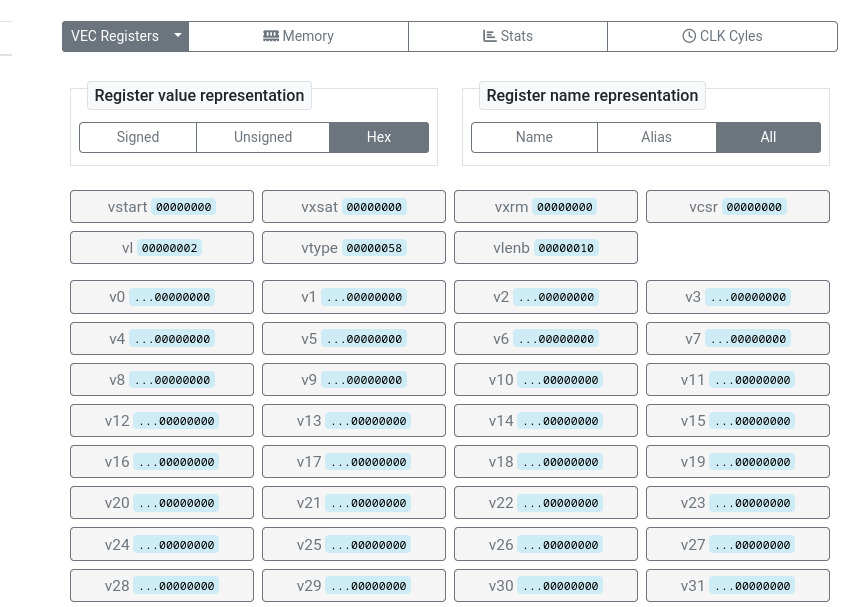
\includegraphics[width=0.6\textwidth]{vec_register_bank.jpg}
    \caption{Pestaña VEC-Registers}\label{fig:register-bank}
\end{figure}

Los registros de control se han colocado en la parte superior del banco de registros. Los registros vectoriales se encuentran inmediatamente debajo. De la misma forma que para los demás registros, se puede seleccionar ver los valores almacenados en forma de valor con signo, valor sin signo y hexadecimal. En los primeros dos casos, se muestran los valores de menor índice del vector; en el caso de la representación en hexadecimal, se muestran los bits menos significativos ya que se corresponden con los primeros elementos del vector (Sección~\ref{subsec:mapping-vector-elements}).

\subsubsection{Pop-over}

El pop-over muestra la información de un registro. Para los registros vectoriales, al ser completamente diferentes a otro tipo de registros, se ha diseñado un componente con otra estructura para lograr una correcta visualización de los elementos almacenados en el vector (Figura~\ref{fig:pop-over}).

El pop-over muestra en la cabecera la configuración de la arquitectura (i.e. SEW y VL). Además permite la visualización de cada uno de los elementos del vector en binario, hexadecimal, entero sin signo y entero con signo. Por último, los elementos de cola se distinguen visualmente al tener un tono más oscuro.

\begin{figure}[H]

    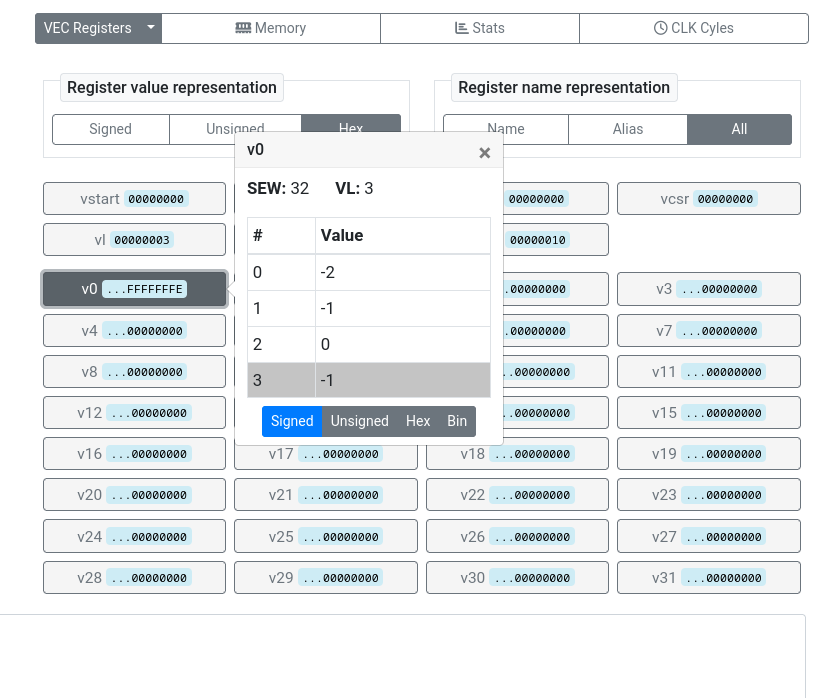
\includegraphics[width=0.6\textwidth]{pop-over.png}
    \caption{Pestaña VEC-Registers}\label{fig:pop-over}
\end{figure}

\subsubsection{Pestañas \textit{Stats} y \textit{CLK Cycles}}

La pestañas \textit{Stats} y \textit{CLK Cycles} muestran diferente información acerca del porcentaje de ejecución de cada uno de los tipos de instrucciones y el número de ciclos de reloj invertido en cada tipo, respectivamente. Estas pestañas se han adaptado para que incluya un nuevo tipo de instrucción: \textit{vector arithmetic instruction} (Figuras~\ref{fig:stats-clk} y~\ref{fig:clk}).

    \begin{minipage}[t]{0.45\textwidth}
        \begin{figure}[H]
            {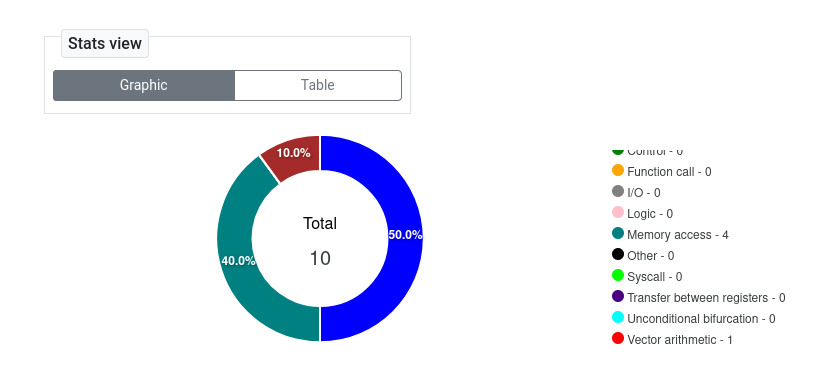
\includegraphics[width=\linewidth]{stats.jpg}}
            \caption{Pestaña \textit{Stats}}\label{fig:stats-clk}
        \end{figure}
    \end{minipage}
    \hfill
    \begin{minipage}[t]{0.45\textwidth}
        \begin{figure}[H]
            {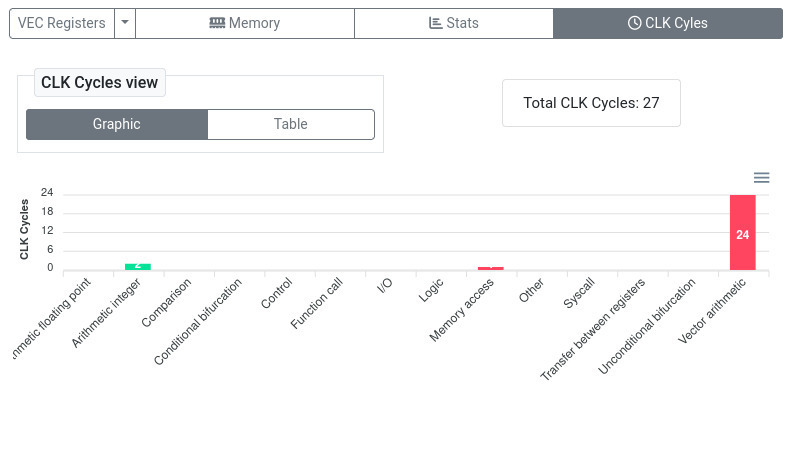
\includegraphics[width=\linewidth]{clk_cycles.jpg}}
            \caption{Pestaña \textit{CLK Cycles}}\label{fig:clk}
        \end{figure}
    \end{minipage}

\section{Despliegue}\label{sec:deploy}

En esta sección se describen los requisitos recomendados para el uso de la aplicación, así como los pasos a seguir para desplegarla. Dado que no se utilizan herramientas diferentes a CREATOR y que, tal y cómo se estableció en los requisitos (sección~\ref{sec:requirements}), se debía conservar la funcionalidad anterior; los requisitos del sistema son los mismos que para la versión de CREATOR disponible el 3 de junio de 2024, fecha en la que se clonó el proyecto para el desarrollo de la propuesta. Estos requisitos se detallan a continuación:

\begin{itemize}
    \item \textbf{Sistema operativo:} Linux, Ubuntu 22.04 LTS, Fedora 39.
    \item \textbf{Procesador:} Intel (R) Core (TM) i3 CPU 8100 @ 3.6Hz o superior.
    \item \textbf{Memoria RAM:} 2 GB o superior.
    \item \textbf{Almacenamiento:} 1 GB de espacio libre en disco duro (espacio recomendado para los navegadores web).
    \item \textbf{Red:} No es necesario internet para lanzar el simulador.
    \item \textbf{Software:} \texttt{Node.js}, \texttt{npm} y alguno de los siguientes navegadores recomendados:
    \begin{itemize}
        \item Google Chrome 70 o superior.
        \item Mozilla Firefox 60 o superior.
        \item Apple Safari 12 o superior.
    \end{itemize}

\end{itemize}

Para desplegar la aplicación es necesario lanzar la aplicación en un servidor \texttt{npx}. Para ello es necesario seguir los siguientes pasos:
\begin{enumerate}
    \item Clonar el respositorio con el código fuente. Se puede hacer mediante el siguiente comando.
\begin{lstlisting}[language=bash, basicstyle=\scriptsize]
git clone https://github.com/CLopMan/creator
\end{lstlisting}
    \item Alojar un servidor local mediante el siguiente comando.
\begin{lstlisting}[language=bash, basicstyle=\scriptsize]
npx http-server creator/ -p 9999
\end{lstlisting}
    \item Acceder al simulador en cualquier navegador de los especificados anteriormente a través de la ip \textit{localhost} y el puerto 9999.
        \begin{figure}[H]
                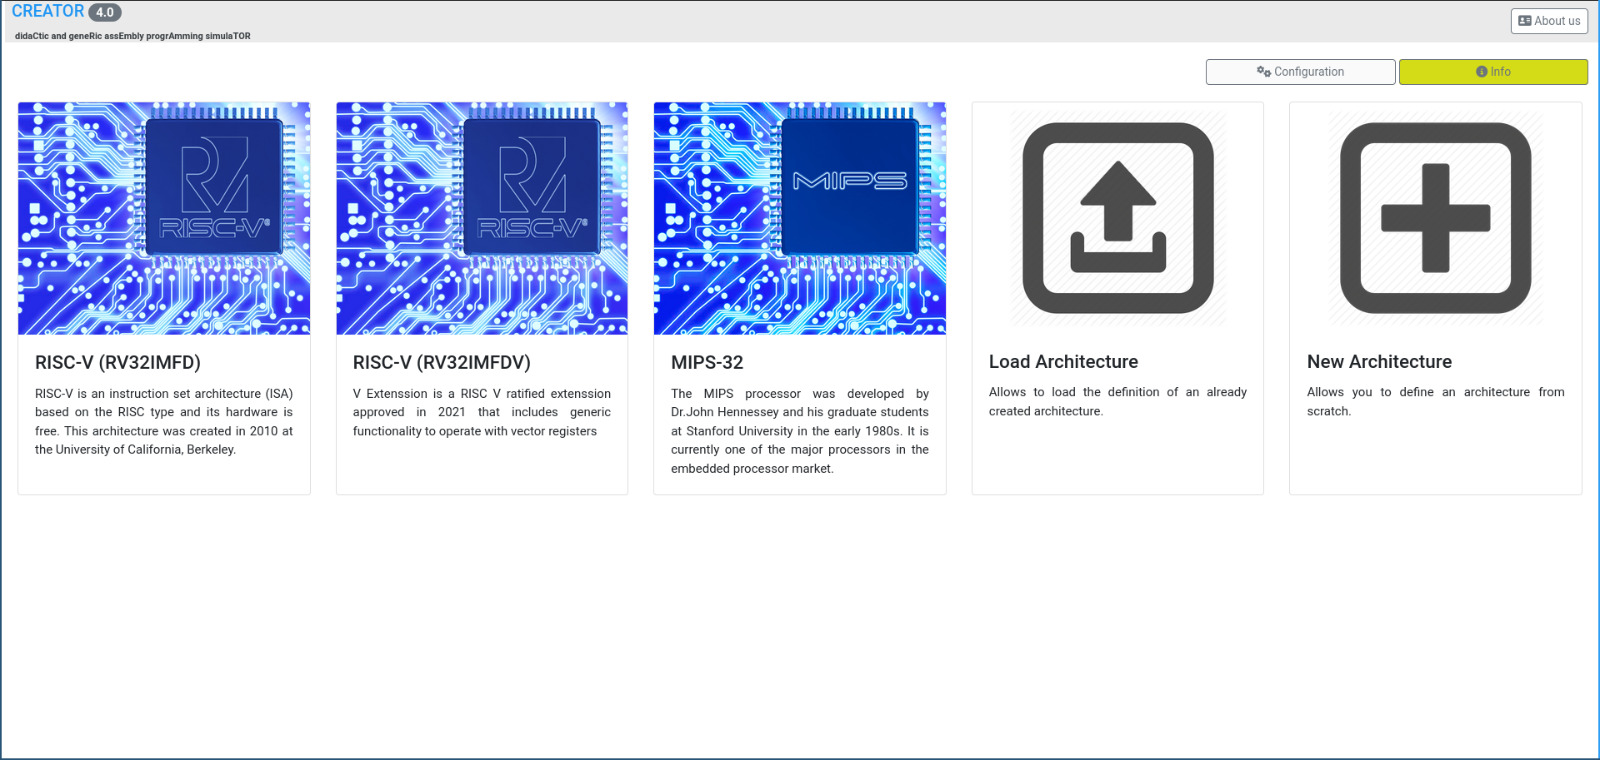
\includegraphics[width=0.9\textwidth]{server_up.png}
                \caption{Página de inicio del simulador}\label{fig:inicio-simulador}
        \end{figure}
    \item Seleccionar la arquitectura RISCV-V (RV32IMFDV).
\end{enumerate}

\section{Resumen}

En este capítulo se han descrito las principales decisiones de implementación de la propuesta, así como la estructura de ficheros. También se han indicado los requisitos mínimos para utilizar la herramienta desarrollada, y los pasos a seguir para desplegarla.
